\documentclass[10pt,a4paper]{article}
\usepackage{nips15submit_e}
\usepackage{amsmath}
\usepackage{mathtools}
\usepackage{amsfonts}
\usepackage{amssymb}
\usepackage{graphicx}
\usepackage{float}
\usepackage{hyperref}
%\usepackage[
%backend=bibtex,
%sorting=unsrt
%]{biblatex}
%\addbibresource{projectsources.bib}
\usepackage{xcolor}

\usepackage[paperwidth=8.5in,paperheight=11in,centering,hmargin=1in,vmargin=1in]{geometry}
\nipsfinalcopy

%\DeclarePairedDelimiter{\norm}{\lVert}{\rVert}
\usepackage{physics}
\newcommand{\R}{\mathbb{R}}
\newcommand{\C}{\mathbb{C}}
\newcommand{\Tau}{\mathcal{T}}

\begin{document}
\title{Image Deblurring and Denoising for Various Fidelity Terms and Regularizers}
\author{
Kelsey Maass, ~Samuel Rudy, ~Kevin Mueller, ~and Riley Molloy\\
University of Washington\\
}

\maketitle

% Introduction
\section{Introduction}

Image denoising and deblurring problems can be modeled with the linear system
\begin{equation}
Ax + w = b,
\end{equation}
where $b$ is the observed image, $w$ is some unknown noise, and $x$ is the true image we would like to recover. For a blurred image we let $A$ represent the blurring process, and for noisy images we let $A$ be the identity matrix. For many inverse problem applications the least squares approximation, 
\begin{equation}
\hat{x}_{LS} = \arg\min_x \| Ax - b \|_2^2 ,
\end{equation}
gives a reasonable solution. Unfortunately, this approach doesn't provide any new information for the denoising problem, and for image deblurring problems $A$ is often ill-conditioned, so the solution is contaminated by round-off error and amplified noise. To illustrate this, we consider the pepper image below. If we blur the image and compute the naive solution $x = A^{-1}b$, the result is obscured by round-off error in the form of ringing artifacts. The result is even worse when we add noise.

\begin{figure}[H]
\centering
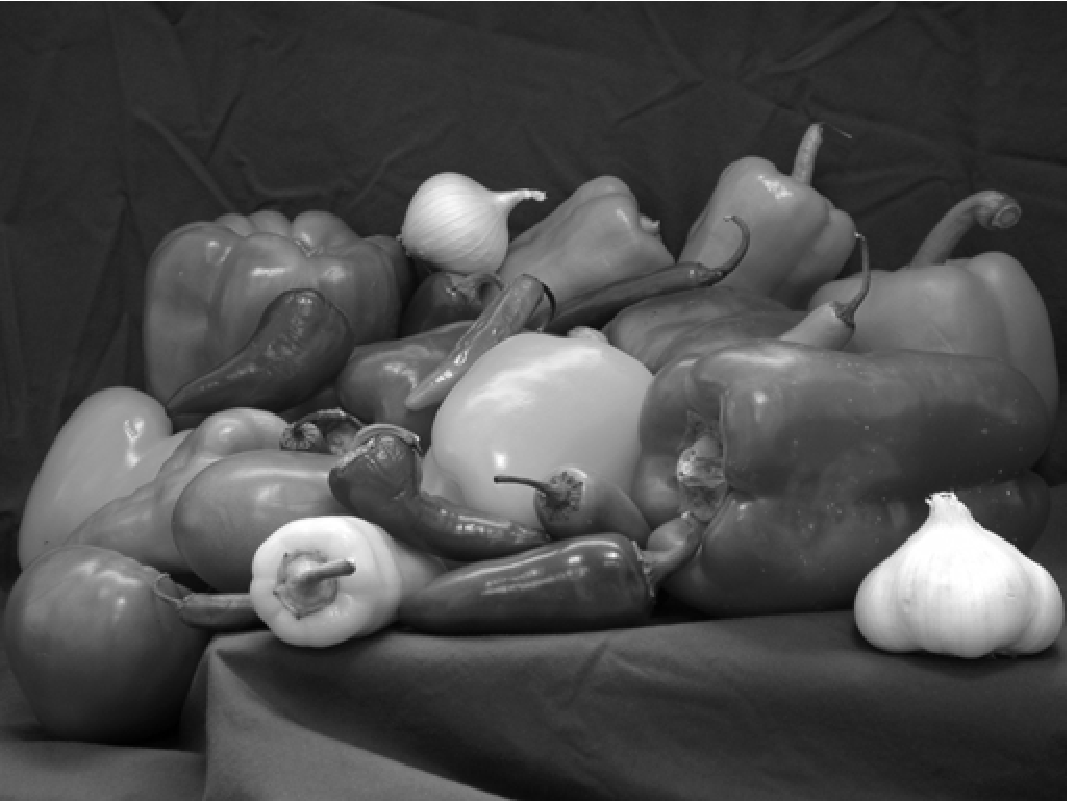
\includegraphics[width=2in]{fig1}
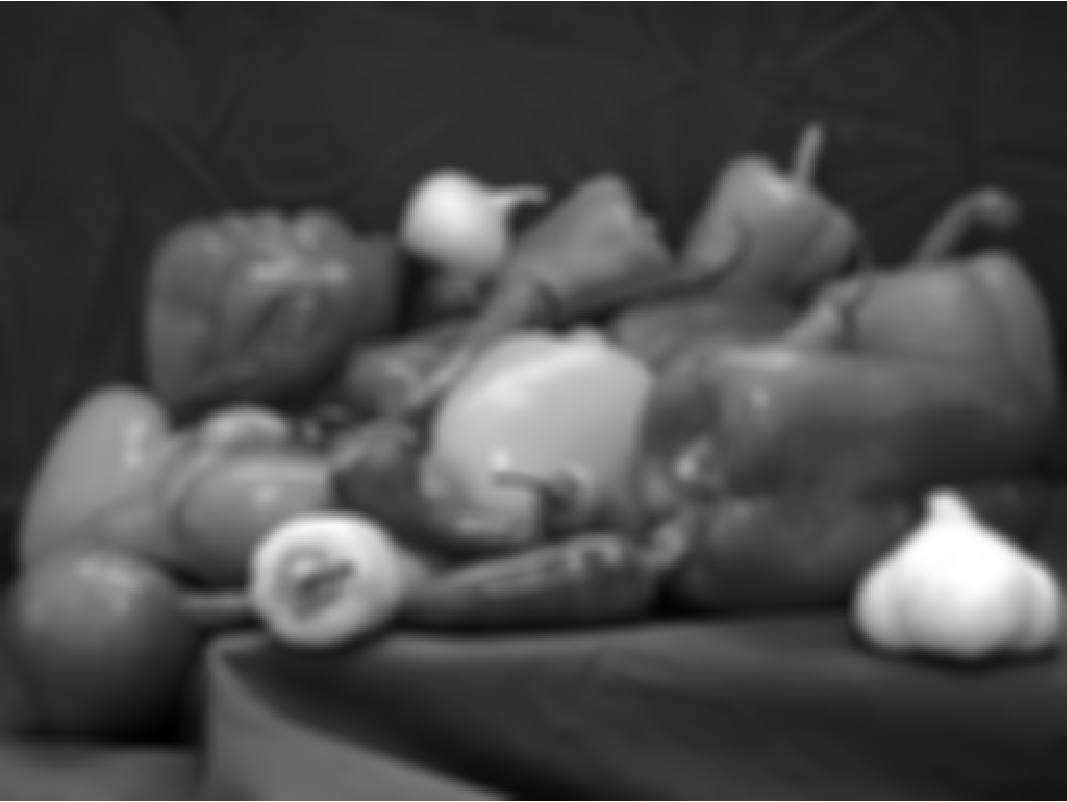
\includegraphics[width=2in]{fig2}
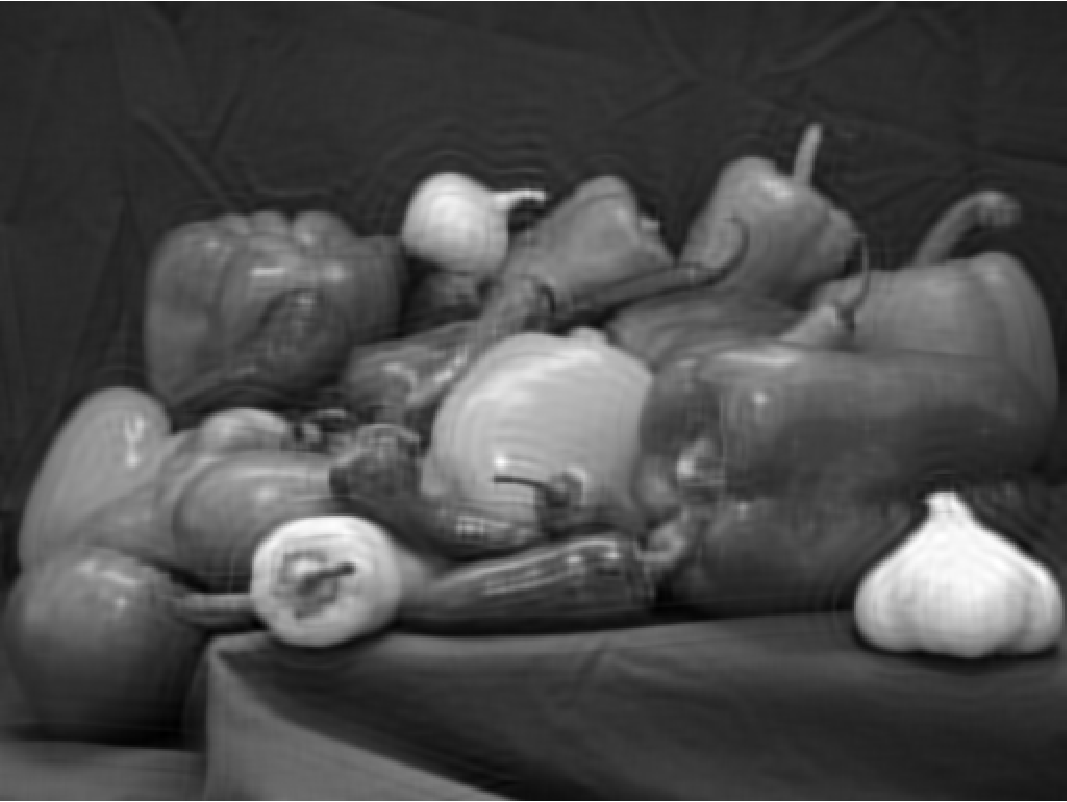
\includegraphics[width=2in]{fig3} \\[1ex]
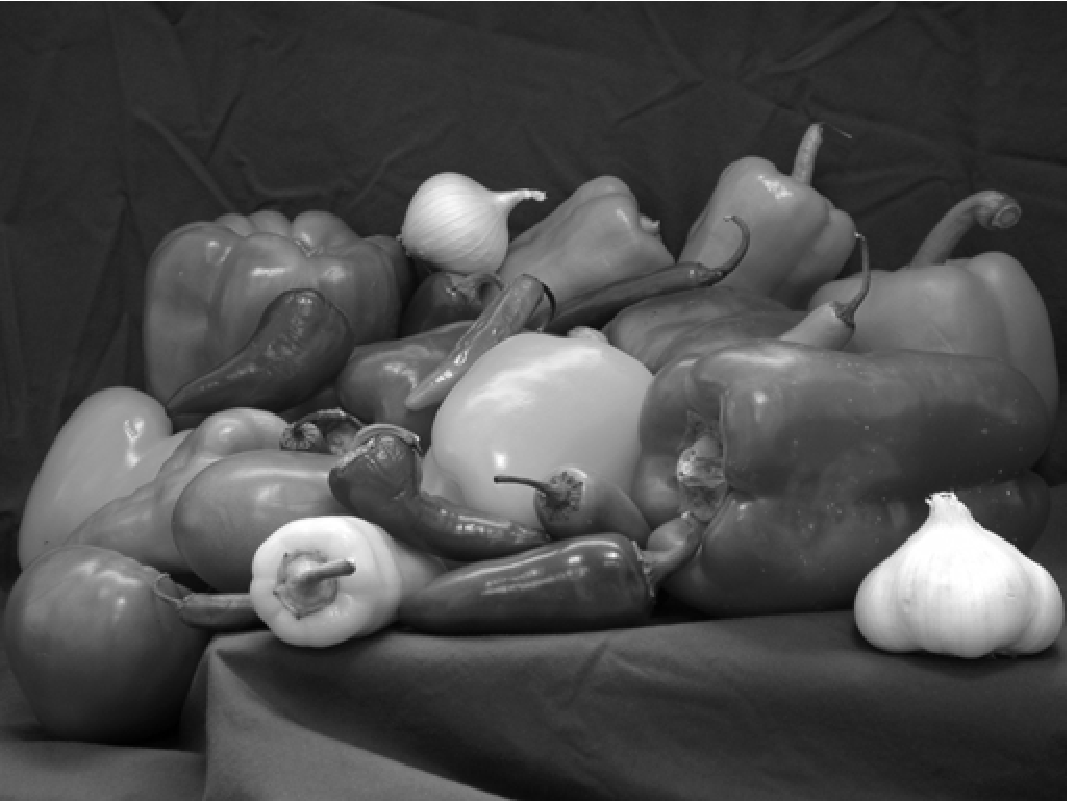
\includegraphics[width=2in]{fig1}
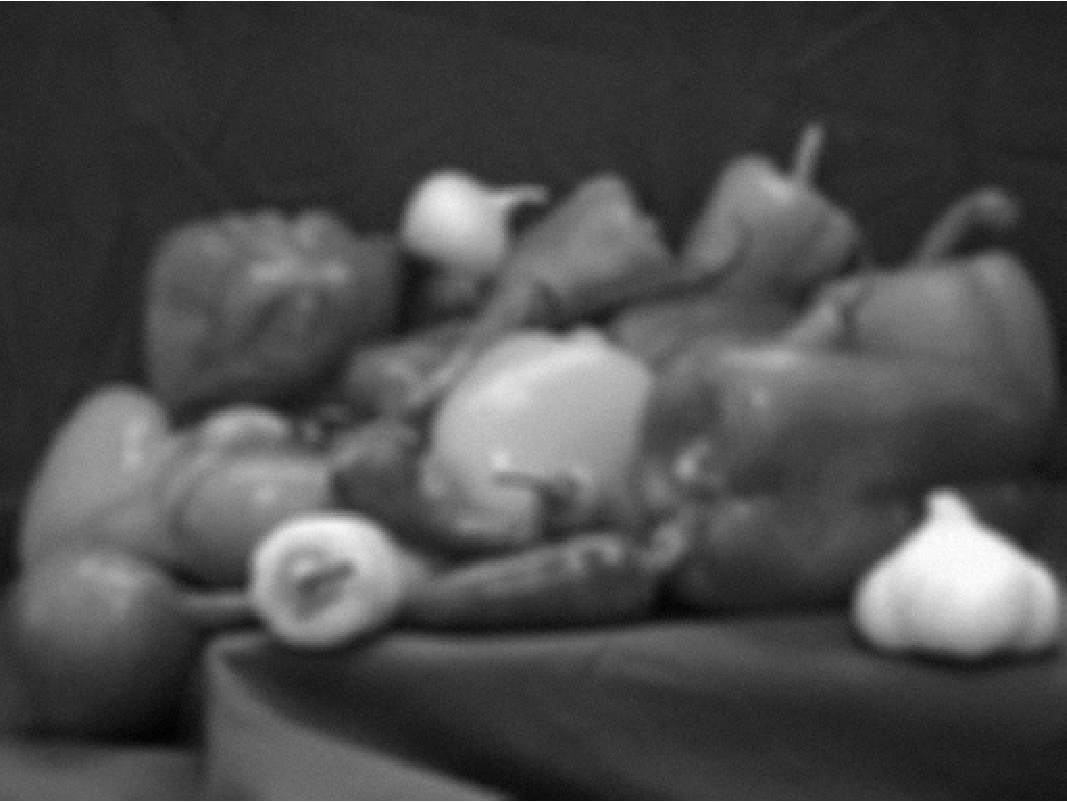
\includegraphics[width=2in]{fig4}
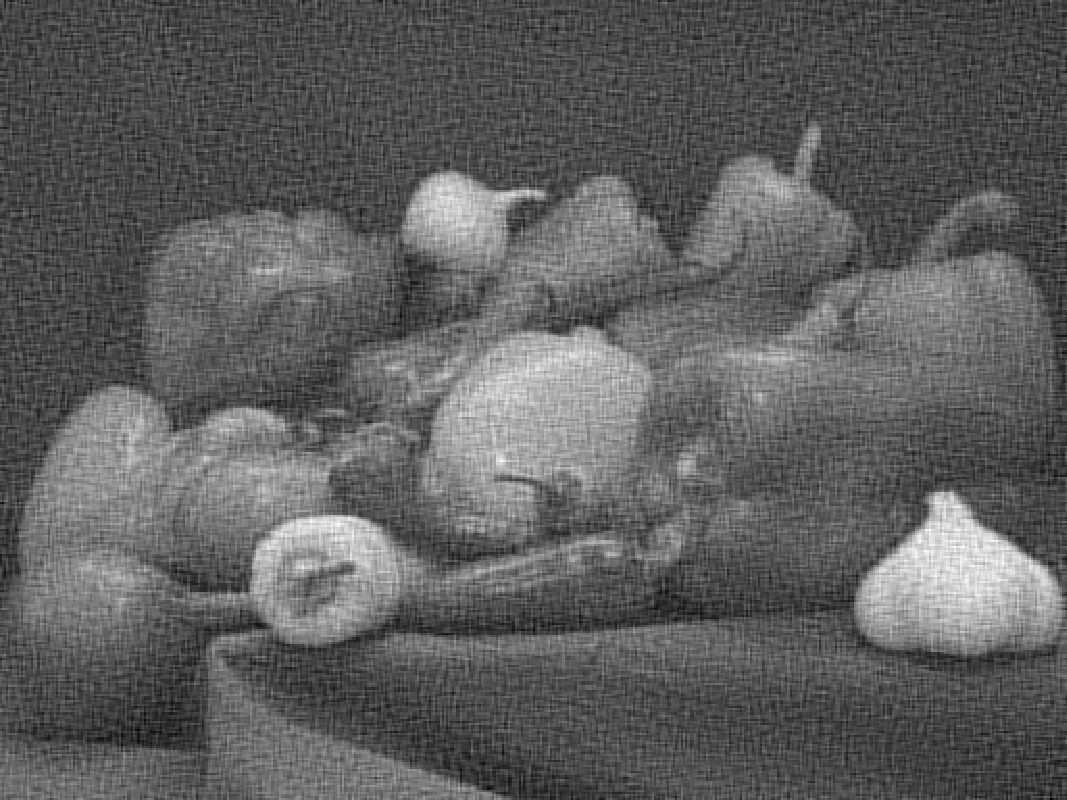
\includegraphics[width=2in]{fig5}
\caption{\small In the top row we observe the naive solution applied to a blurred image, including the true image $x$ (left), the blurred image $b$ (middle), and the recovered image $A^{-1}b$. On the bottom row, we see the effects of adding noise illustrated by the true image $x$ (left), the blurred and noisy image $b-w$ (middle), and the recovered image $A^{-1}(b-w)$.}
\end{figure}

In order to stabilize the solution, a variety of regularizers can be used which exploit features of the true image such as smoothness or sparsity in a wavelet domain. This results in the problem formulation
\begin{equation}
\hat{x} = \arg\min_{x} \| Ax - b \|_2^2 + \lambda R(x),
\end{equation}
where the parameter $\lambda > 0$ is chosen to balance the tradeoff between fidelity to the model and the assumed feature. In this paper we compare two choices for the regularization term, 
\begin{align}
&\text{Total variation regularization:} &\hat{x}_{TV} = \arg\min_x \| Ax - b \|_2^2 + 2\lambda \| x \|_{TV} , \\
&\text{and } L_1 \text{ regularization:} &\hat{x}_{L1} = \arg\min_x \| Ax - b \|_2^2 + \lambda \| Wx \|_1  ,
\end{align}

which are explored by Beck and Teboulle in \cite{TV} and \cite{FISTA} respectively.

It is also known that the 2-norm penalty is extremely sensitive to outliers. While this does not pose problems for images with Gaussian noise, which may result from atmospheric turbulence, it becomes an issues for images with noise from heavier tailed distributions, such as the Student's t-distribution, which could result from a dirty camera lens. Therefore we also consider different choices for the fidelity term which are less sensitive to outliers than the 2-norm penalty, including the Huber norm
\begin{equation}
h_{\gamma}(x) = \min_y \frac{1}{2} \| x - y \|^2 + \gamma \| y \|_1,
\end{equation}
and the function
\begin{equation}
g_{\gamma}(x) = \frac{1}{\gamma} \sum_i \log\left(\cosh\left(\gamma x_i\right)\right).
\end{equation}


% Background
\section{Background of Methodology and Implementation}
The general approach of to an image deblurring or denoising problem is the minimization of a loss function of the form
\begin{equation} \label{general}
 \min_x f(\mathcal{A}(x) -b) + g(x),
\end{equation}
where $\mathcal{A}(x)$ is a convolution of the desired image $x$ with a gaussian kernel creating a blur,  $f : \R^{m \times n} \rightarrow [0, \infty)$ represents some continuous measure of distance between the corrupt image $b$ and the desired image $x$, and $g:\R^{m \times n} \rightarrow [0,\infty)$ is some regularization on the allowed amount of noise in $x$. The term $f(\mathcal{A}(x)-b)$ is referred to as the \emph{fidelity term}, and the term $g(x)$ is referred to as the \emph{regularization}. We can represent the blurring convolution $\mathcal{A}(\cdot): \R^{m \times n} \rightarrow \R^{m \times n}$ by left matrix multplication with some matrix $A$, so we do so for convenience from here forward. In addition, since we require some pixel value $x_{ij} \in [0,1]$, we can add an additional term to the loss function as
\begin{equation} \label{loss}
 L_b(x) = f(Ax-b) + g(x) + \delta(x | [0,1] ),
\end{equation}
where $\delta(x | [0,1])$ is an indiciator function for the unit interval. 

\emph{here we can explain the general prox-gradient approach, and go into details for specific cases in the following subsections}

% TV Regularization
\subsection{Total Variation Regularization}
The usual Total-Variation deblurring model, as seen in (BECK/TOUBELLE REF) can be formulated as 
\begin{equation} \label{tv_orig}
\min_{x} \norm{ Ax - b }^2 + 2 \lambda \mathrm{TV}(x),
\end{equation}
where $\norm{\cdot}$ is taken as either a Frobenius norm or a 2-norm, depending on applications,  $\lambda>0$ is a regularization parameter, and $\mathrm{TV}(x)$ is the Total-Variation semi-norm. Two choices similar choices exist for the TV-norm: the so-called isotropic type, and the $l_1$ type. In this work, we work exclusively with the $l_1$-based TV-norm, defined as 
$$ TV_{l_1}(x) = \sum_{i=1}^{m-1} \sum_{j=1}^{n-1} \left( \abs{x_{i,j}  - x_{i+1,j} } + \abs{ x_{i,j} - x_{i,j+1}  } \right) + \sum_{i=1}^{m-1} \abs{ x_{i,n} - x_{i+1,n} } + \sum_{j=1}^{n-1} \abs{ x_{m,j} - x_{m,j+1 } },$$ for $x \in \R^{m \times n},$ and where the reflexive boundary conditions
\begin{align*}
x_{m+1,j} - x_{m,j} &= 0, \textrm{ for all }j \\
 x_{i,n+1} - x_{i,n} &= 0, \textrm{ for all }i
\end{align*}
are assumed. Our approach considers a more general problem
\begin{equation} \label{tv_ours}
\min_{x} f(Ax - b ) + 2 \lambda \mathrm{TV}_{l_1}(x),
\end{equation}
where $f: \R^{m \times n} \rightarrow [0,\infty)$ is any continuous functional which gives a measurement of the size of the fidelity term.


% 1-Norm Wavelet Regularization
\subsection{1-Norm Wavelet Regularization}


\section{Testing}

\subsection{Something}


\subsection{Something Else}



\section{Results}

\section{Discussion}

%\printbibliography[title={Sources}]
\bibliographystyle{unsrt}
\bibliography{sources}


\end{document}